%\documentclass[12pt]{article}
\documentclass[a4paper]{article}
\usepackage{amsmath,amsfonts,amssymb}
\usepackage[utf8]{inputenc}
\usepackage{graphicx}
\usepackage{verbatim}
\usepackage{float}
\usepackage[makeroom]{cancel} %
\usepackage[english]{babel}
\usepackage{textcomp}
\usepackage{gensymb} %
\usepackage{color}
\usepackage{subcaption}
\usepackage{caption}
%\usepackage{hyperref}
%\usepackage{physics}
%\usepackage{dsfont}
%\usepackage{amsfonts}
\usepackage{listings}
\usepackage{multicol}
\usepackage{units}
\usepackage{bm}

% From Eirik's .tex
\usepackage{epstopdf}
\usepackage{cite}
\usepackage{braket}
\usepackage{url}
\bibliographystyle{unsrt}

\usepackage{algorithmicx}
\usepackage{algorithm}% http://ctan.org/pkg/algorithms
\usepackage{algpseudocode}% http://ctan.org/pkg/algorithmicx

\usepackage[margin=1cm]{caption}
\usepackage[outer=1.2in,inner=1.2in]{geometry}
% For writing full-size pages
%\usepackage{geometry}
%\geometry{
%  left=5mm,
%  right=5mm,
%  top=5mm,
%  bottom=5mm,
%  heightrounded,
%}

% Finding overfull \hbox
\overfullrule=2cm

\lstset{language=IDL}
 %\lstset{alsolanguage=c++}
\lstset{basicstyle=\ttfamily\small}
 %\lstset{backgroundcolor=\color{white}}
\lstset{frame=single}
\lstset{stringstyle=\ttfamily}
\lstset{keywordstyle=\color{red}\bfseries}
\lstset{commentstyle=\itshape\color{blue}}
\lstset{showspaces=false}
\lstset{showstringspaces=false}
\lstset{showtabs=false}
\lstset{breaklines}
\lstset{aboveskip=20pt,belowskip=20pt}

\lstset{basicstyle=\footnotesize, basewidth=0.5em}
\lstdefinestyle{cl}{frame=none,basicstyle=\ttfamily\small}
\lstdefinestyle{pr}{frame=single,basicstyle=\ttfamily\small}
\lstdefinestyle{prt}{frame=none,basicstyle=\ttfamily\small}
% \lstinputlisting[language=Python]{filename}


\definecolor{codepurple}{rgb}{0.58,0,0.82}
\definecolor{backcolour}{rgb}{0.95,0.95,0.92}
\definecolor{dkgreen}{rgb}{0,0.6,0}
\definecolor{gray}{rgb}{0.5,0.5,0.5}
\definecolor{magenta}{rgb}{0.58,0,0.82}

\lstdefinestyle{pystyle}{
  language=Python,
  aboveskip=3mm,
  belowskip=3mm,
  columns=flexible,
  basicstyle={\small\ttfamily},
  backgroundcolor=\color{backcolour},
  commentstyle=\color{dkgreen},
  keywordstyle=\color{magenta},
  numberstyle=\tiny\color{gray},
  stringstyle=\color{codepurple},
  basicstyle=\footnotesize,
  breakatwhitespace=false,
  breaklines=true,
  captionpos=b,
  keepspaces=true,
  numbers=left,
  numbersep=5pt,
  showspaces=false,
  showstringspaces=false,
  showtabs=false,
  tabsize=2
}

\lstset{language=[90]Fortran,
  basicstyle=\small\ttfamily,
  keywordstyle=\color{red},
  commentstyle=\color{blue},
  stringstyle=\color{dkgreen},
  morecomment=[l]{!\ },
  numbers=left,
  numbersep=5pt
}

%%%%%%%%%%%%%%%%%%%%%%%%%%%%%%%%
% Self made macros here yaaaaaay
\newcommand\answer[1]{\underline{\underline{#1}}}
\newcommand\pd[2]{\frac{\partial #1}{\partial #2}}
\newcommand\red[1]{\textcolor{red}{\textbf{#1}}}
\newcommand\numberthis{\addtocounter{equation}{1}\tag{\theequation}}
% Usage: \numberthis \label{name}
% Referencing: \eqref{name}

% Some matrices
\newcommand\smat[1]{\big(\begin{smallmatrix}#1\end{smallmatrix}\big)}
\newcommand\ppmat[1]{\begin{pmatrix}#1\end{pmatrix}}

%%%%%%%%%%%%%%%%%%%%%%%%%%%%%%%%%
% Eirik's self made macros
\newcommand{\s}{^{*}}
\newcommand{\V}[1]{\mathbf{#1}}
\newcommand{\husk}[1]{\color{red} #1 \color{black}}
\newcommand{\E}[1]{\cdot 10^{#1}}
\newcommand{\e}[1]{\ \text{#1}}
\newcommand{\tom}[1]{\big( #1 \big)}
\newcommand{\Tom}[1]{\Big( #1 \Big)}
\newcommand{\tomH}[1]{\big[ #1 \big] }
\newcommand{\TomH}[1]{\Big[ #1 \Big]}
\newcommand{\tomK}[1]{ \{ #1 \} }
\newcommand{\TomK}[1]{\Big\lbrace #1 \Big\rbrace}
\newcommand{\bigabs}[1]{\left| #1 \right|}

% Practical macros for FYS-STK4155
\newcommand{\XX}{\mathbf{X}}
\newcommand{\II}{\textbf{I}}
\newcommand{\T}{\mathsf{T}}

\newcommand{\Ey}{\mathbb{E}[\bm{\tilde y}]}
\newcommand{\xx}{\mathbf{x}}
\newcommand{\ee}{\bm{\epsilon}}
\newcommand{\yy}{\bm{\tilde y}}


% Section labeling
%\usepackage{titlesec}% http://ctan.org/pkg/titlesec
%\renewcommand{\thesubsection}{\arabic{subsection}}

% Title/name/date
\title{FYS-STK4155: Project 1}
\author{Simen Nyhus Bastnes}
\date{10. October 2020}

\begin{document}
\maketitle
%%%%%%%%%%%%%%%%%%%%%%%%%%%%%%%%%%%%%%%%%%%%%%%%%
\begin{abstract}
In this project, we will study various methods of linear regression, namely the Ordinary Least Squares method, Ridge, and Lasso regression, as well as investigate resampling the data via Bootstrapping and $k$-fold Cross-Validation. The data we will be looking at is the so-called Franke function, as well as terrain elevation data from a region south-east in Norway. The Franke function gives us a way of testing our implementation before moving on to the more complex terrain data. For the Franke function, we found that Ridge regression performed the best for both Bootstrap and Cross-validation, when it comes to both accuracy and stability. Cross-validation gave the lowest estimate for the error. For the terrain data, we looked at a single patch from the map, and found that OLS performed a decent bit better than Ridge and Lasso, but since we did not reach the overfitting regime, the results might change if we had used a higher $p_{\text{max}}$.

%The goal of this project is to do linear regression with bootstrapping and cross-validation on the Franke function and real data.
\end{abstract}
%%%%%%%%%%%%%%%%%%%%%%%%%%%%%%%%%%%%%%%%%%%%%%%%%%%%%%%%%%%%%%%%%%%%%%%%%%%%%%%%%%%%%%%%%%
%%%%%%%%%%%%%%%%%%%%%%%%%%%%%%%%%%%%%%%%%%%%%%%%%%%%%%%%%%%%%%%%%%%%%%%%%%%%%%%%%%%%%%%%%%
\section{Introduction}
% not good enough maybe check first sentence

With the emergence of more powerful computers, the field of machine learning is steadily becoming an integral part of both business and many fields of science. While many of the concepts and algorithms used in machine learning today has been known for a long time, some of them have simply been too computationally expensive to do efficiently. Linear regression is one of the simplest and most-studied forms of machine learning, and provides a good introduction to concepts commonly used in machine learning. 
\\\\
In this project, we will look at three different methods of regression analysis and compare how they fare against each other. The methods we will be using is the Ordinary Least Squares method, Ridge regression, and Lasso regression. We will also see how resampling the data affects the results from the regression methods, by implementing the Bootstrap algorithm and the $k$-fold Cross-Validation.
\\\\
There are two different data sets that will be studied in this project. The first, is the Franke function from \cite{Franke}, as well as terrain data for a region in Norway taken from \cite{terrain}. First, in Chapter \ref{chap:theory} we will introduce the theory behind linear regression, as well as the the regression methods and resampling methods employed later in the project. In Chapter \ref{chap:implement} we go through the implementation of the methods, explaining how the code is structured and used. Then, in Chapter \ref{chap:results} we go through the results of both the Franke function and the terrain data, while discussing them. %discussing them in more detail in Chapter \ref{chap:discussion}. 
Lastly, we conclude our findings in Chapter \ref{chap:conclusion}.

%%%%%%%%%%%%%%%%%%%%%%%%%%%%%%%%%%%%%%%%%%%%%%%%%%%%%%%%%%%%%%%%%%%%%%%%%%%%%%%%%%%%%%%%%%
%%%%%%%%%%%%%%%%%%%%%%%%%%%%%%%%%%%%%%%%%%%%%%%%%%%%%%%%%%%%%%%%%%%%%%%%%%%%%%%%%%%%%%%%%%
\section{Theory} \label{chap:theory}
%For the derivation of the OLS method, Ridge, and Lasso regression, we will follow Chapter 2.3 and 3.4 of Hastie et al. \cite{Hastie}
\subsection{Linear regression} \label{sec:linreg}
%Assume we have a data set $\bm{y}$
%At its core, x
Linear regression is a method of fitting a set of $p$ \textit{predictors} $\bm{X}$ to a data set $\bm{y}$, while minimizing the error between the \textit{response} $\bm{\tilde y}$ and the actual data $\bm{y}$. For each of the $n$ samples $y_i$ in the data set the relationship between the response and the predictors $\bm{X}_i$ is modeled in a linear fashion, giving us the following matrix equation
\begin{align*}
	\mathbf{y} &= \XX\beta + \bm{\epsilon}
\end{align*}
where $\beta = (\beta_0, \beta_1, ..., \beta_ {p-1})^\T$ are the regression parameters we are trying to estimate, one for each predictor, and $\bm{\epsilon}$ is the error in our approximation. The matrix $\XX$ is often called the design matrix, and the equation can be written a bit more explicitly as
\begin{align*}
	y_i &= \beta_0 + X_{i,1}\beta_1 + ... + X_{i,p-1}\beta_{p-1} + \epsilon_i
\end{align*}
Exactly what each predictor is can vary a lot from case to case, and how the design matrix is set up is important for the accuracy of the fit. In our case, we will focus on a form of linear regression where the predictors is on the form of a polynomial in the input parameters. In the case where we have a data set $\bm{y}(\bm{x})$, the design matrix can for example be written on the form of
\begin{align*}
	\XX &= (\bm{x}^0, \bm{x}^1, ... , \bm{x}^{p-1})
\end{align*} 
With that said, we still need some way to find the $\beta$'s that fit the data best, and we will now look at three ways to try to do this.
% This is done
%Assuming that we have a set of \textit{response} allalal
%linear regresssion Fitting a continuous function with linear parameterization in terms of the parameters $\beta$.
%Giving us the matrix equation
%Linear regression is a way of modeling a relationship between the response $y_i$ and some amount of explanatory variables $x_i$ in a linear fashion. Assume we have 
%\begin{align*}
%	\mathbf{y} &= \beta_0 + \sum_{i=1}^{p}\XX_i\beta_i + \mathbf{\varepsilon}_i
%	\mathbf{y} &= \XX\beta + \mathbf{\varepsilon}\\
%	\mathbf{y}_i &= \beta_0 + \sum_{j=1}^{p}\XX_{ij}\beta_j + \mathbf{\varepsilon}_i	
%\end{align*}

\subsubsection{Ordinary least squares}
Following Chapter 2.3 of Hastie et al. \cite{Hastie}, in order to find the optimal regression parameters $\beta$, the OLS method minimizes the residual sum of squares
\begin{align*}
	\text{RSS}(\beta) &= \sum_{i=1}^N(y_i-x_i^T\beta)^2
\end{align*}
With $\bm{y}$ as the vector containing all $N$ $y_i$, and $X$ an $N\times p$ matrix as shown in section \ref{sec:linreg}, this can be written as
\begin{align*}
	\text{RSS}(\lambda) &= (\bm{y} - \XX\beta)^\T(\bm{y}-\XX\beta)
\end{align*}
Differentiating with respect to $\beta$ we get
\begin{align*}
	\pd{\text{RSS}}{\beta} &= X^\T(\bm{y}-\XX\beta)
\end{align*}
In order to find an optimal $\beta$, this has to be zero
\begin{align*}
	\XX^\T(\bm{y}-\XX\beta) &= 0\\
	\XX^\T\XX\beta &= \XX^T\bm{y}
\end{align*}
Finally giving us the expression for the optimal regression parameters
\begin{align*}
	\beta &= (\XX^\T\XX)^{-1}\XX^\T\bm{y}
\end{align*}
assuming that $\XX^\T\XX$ is invertible.

\subsubsection{Ridge regression}
Ridge regression is an example of a so-called shrinkage method, which shrinks the regression coefficients by adding a small penalty proportional to their size.
\begin{align*}
	\beta^{\text{Ridge}} &= \underset{\beta\in \mathbb{R}^{p}}{\text{min}}\frac{1}{n}||\bm{X}\beta - \bm{y}||^2_2 + \lambda||\beta||^2_2
\end{align*}
where $\lambda$ is a regularization parameter that controls the amount of shrinkage, and we $||\beta||^2_2 \leq t$ where $t$ is a finite number larger than zero. The higher $\lambda$, the more shrinkage occurs. This can be shown to give the Ridge solution
\begin{align*}
	\beta^{\text{Ridge}} &= (\XX^\T\XX + \lambda I)^{-1}\XX^\T\bm{y}
\end{align*}
The aim with Ridge regression is to limit the potential problems with singularities when computing the inverse of $\XX^\T\XX$, which can be a problem when there are many correlated variables.
\subsubsection{Lasso regression}
Lasso regression is another shrinkage method, with a slightly different optimization equation compared to Ridge regression
\begin{align*}
	\beta^{\text{Lasso}} &= \underset{\beta\in \mathbb{R}^{p}}{\text{min}}\frac{1}{n}||\bm{X}\beta - \bm{y}||^2_2 + \lambda||\beta||_1
\end{align*}
where $||\beta||_1$ is the $L_{1}$ norm.
\subsection{Bias-Variance decomposition}
Starting from the so-called cost function, we want to derive an expression for the variance and bias for the predicted values $\bm{\tilde y}$
\begin{align*}
	C(\XX, \beta) &= \frac{1}{n}\sum_{i=0}^{n-1}(y_i-\tilde y_i)^2 = \mathbb{E}[(\bm{y}-\bm{\tilde y})^2]
\end{align*}
assuming that the true data is generated from a noisy model $\bm{y} = f(\bm{x})+\bm{\epsilon}$ where $\epsilon$ is normally distributed with zero mean and standard deviation $\sigma^2$, we get
\begin{align*}
\mathbb{E}[(\bm{y}-\bm{\tilde y})^2] &= \mathbb{E}\Big[(f+\ee - \yy)^2\Big]\\
\intertext{We add and subtract $\Ey$ to the expression}
&= \mathbb{E}\Big[(f + \ee - \yy + \Ey - \Ey)^2\Big]\\
&= \mathbb{E}\Big[(f-\Ey) - (\yy - \Ey) + \ee)^2\Big]\\
\intertext{Expanding the expression gives us}
&= \mathbb{E}\Big[(f-\Ey)^2 + (\yy-\Ey)^2 + \ee^2 - 2(f-\Ey)(\yy-\Ey) \\
&+ 2(f-\Ey)\ee - 2(\yy-\Ey)\ee \Big]\\
\intertext{We can use that the mean of $\ee$ is zero, thus making the last two terms vanish $\mathbb{E}[\ee] = 0$}
&= \mathbb{E}\Big[(f-\Ey)^2 + (\yy-\Ey)^2 + \ee^2 - 2(f-\Ey)(\yy-\Ey) \Big]
\end{align*}
For this to give the results we want, the last term should also be zero, but I don't see how, and often the derivation is just skipped over, or with confusing notation. Assuming it is zero, we get
\begin{align*}
\mathbb{E}[(\bm{y}-\bm{\tilde y})^2] &= \mathbb{E}[(f-\Ey)^2] + \mathbb{E}[(\yy-\Ey)^2] + \mathbb{E}[\ee^2]\\
\intertext{Using that $\mathbb{E}[\ee^2] = \sigma^2$, we get the final expression for the bias-variance decomposition}
\mathbb{E}[(\bm{y}-\bm{\tilde y})^2] &= \mathbb{E}[(f-\Ey)^2] + \mathbb{E}[(\yy-\Ey)^2] + \sigma^2\\
\end{align*}
Where the left-hand side is the so-called mean squared error (henceforth referred to as MSE), the first term is the bias term, which measures how much the our model $\yy$ differs from the true model $f(\xx)$. The second term is the variance of our model, while the third term is the noise. High bias indicates underfitting, and the model is not complex enough to capture the relevant features, while high variance can indicate that the model is overfitting, and adjusting to the smallest variations in the data set.\\\\
Thus, our goal in this project is to try to find the middle ground between high bias and high variance, and that will be the point where the MSE is the lowest, and thus it makes a lot of sense to use it as a measure for how good our model is.
\\\\
The MSE can be written more explicitly as
\begin{align*}
\text{MSE}(\bm{y},\yy) &= \frac{1}{n}\sum_{i=0}^{n-1}(y_i-\tilde y_i)^2 
\end{align*}
Another way of assessing the results would be the $R^2$ score
\begin{align*}
R^2(\bm{y},\yy) &= 1-\frac{\sum_{i=0}^{n-1}(y_i - \tilde y_i)^2}{\sum_{i=0}^{n-1}(y_i - \bar{\bm{y}})^2}
\end{align*}
where
\begin{align*}
\bar{\bm{y}} &= \frac{1}{n}\sum_{i=0}^{n-1}y_i
\end{align*}
\subsection{Confidence intervals}
For the OLS and Ridge regression cases, it is possible to derive the variance of $\beta$ (a proper derivation is given in \cite{vanwieringen2020lecture}), and thus the confidence intervals as well. For the OLS method, the variance is given by
\begin{align*}
	\text{Var}(\beta) &= \sigma^2(\XX^\T\XX)^{-1}
\end{align*}
where $\sigma^2$ is the estimated variance of $y$ given by %TODO a eiwahjhlkwa hw
\begin{align*}
	\sigma^2 &= \frac{1}{N-p-1}\sigma_{i=1}^N(y_i-\tilde y_i)^2
\end{align*}
Taking the square root of the diagonal of $(\XX^\T\XX)^{-1}$ gives us an estimate of the variance of the $j$-th regression coefficient
\begin{align*}
	\sigma^2(\beta_j) &= \sigma^2\sqrt{[\XX^\T\XX]^{-1}_{jj}}
\end{align*}
Letting us construct the 95\% confidence intervals by
%The confidence interval is then given by
\begin{align*}
	\text{CI}(\beta_j) &= \bigg[\beta_j - 2\sqrt{\sigma_2(\beta_j)}\:,\;\; \beta_j + 2\sqrt{\sigma_2(\beta_j)}\bigg]
\end{align*}
%Both can be found in van vieringen | also lecture notes...... 36
Similarly, the variance for $\beta$ for Ridge regression can be found to be
\begin{align*}
\text{Var}[\beta^{\text{Ridge}}] &= \sigma^2[\XX^\T\XX + \lambda\II]^{-1}
\XX^\T \XX[(\XX^\T \XX + \lambda \II)^{-1}]^\T
\end{align*}
and confidence interval can be constructed following the same steps as done above for OLS.% the same way as above for OLS.

\subsection{Resampling methods}
In order to assess our models properly, we will be using some form of resampling. Specifically, we will be looking at the Bootstrap, and the standard $k$-fold Cross-validation resampling methods.
\subsubsection{Bootstrap}
The basic concept of the Bootstrap resampling method is to create new data sets by drawing samples (with replacement) from the training data set. Algorithm \ref{alg:bootstrap} shows the Bootstrap method given a data set $\mathcal{L}$ consisting of the data $\XX_{\mathcal{L}} = \{(y_j, \bm{x}_j), j= 0 \,...\, n-1\}$
\begin{algorithm}[H]
\caption{Bootstrap}
\begin{algorithmic}[1]
\State Split the data set $\XX_{\mathcal{L}}$ into training $\XX_{\mathcal{L},\text{train}}$ and test data sets $\XX_{\mathcal{L},\text{test}}$
\For{$i = 0$, $N_{\text{bs}}-1$}
\State Create a new data set $\XX_{\mathcal{L},i}$ by drawing samples with replacement from  $\XX_{\mathcal{L},\text{train}}$.
\State Fit the model using $\XX_{\mathcal{L},i}$.
\State Evaluate the model on the test set $\XX_{\mathcal{L},\text{test}}$ and store the results.
\EndFor
\State Assess the model by looking at the distribution of computed quantities, for example looking at the mean of the MSE.
\end{algorithmic}
\label{alg:bootstrap}
\end{algorithm}

\subsubsection{Cross-validation}
Cross-validation is a resampling method where (in the case of $k$-fold CV) the data set is split into $k$-folds of training and test data sets. Algorithm \ref{alg:cv} shows the standard $k$-fold cross-validation.
\begin{algorithm}[H]
\caption{$k$-fold Cross-Validation}
\begin{algorithmic}[1]
\State Shuffle the data set $\XX_{\mathcal{L}}$ randomly.
\State Split the data set $\XX_{\mathcal{L}}$ into $k$ folds/subsets $\{\XX_{\mathcal{L},i}, i=0\,...\,k-1\}$.
\For{$i = 0$, $k-1$}
\State Set $\XX_{\mathcal{L},i}$ as the test data set and the rest of the folds as the training set.
\State Fit the model using the training data set as defined above.
\State Evaluate the model on the $i$-th test set $\XX_{\mathcal{L},i}$ and store the results.
\EndFor
\State Assess the model by looking at the distribution of computed quantities.%, for example looking at the mean of the MSE.
\end{algorithmic}
\label{alg:cv}
\end{algorithm}
%If we had

%%%%%%%%%%%%%%%%%%%%%%%%%%%%%%%%%%%%%%%%%%%%%%%%%%%%%%%%%%%%%%%%%%%%%%%%%%%%%%%%%%%%%%%%%%
%%%%%%%%%%%%%%%%%%%%%%%%%%%%%%%%%%%%%%%%%%%%%%%%%%%%%%%%%%%%%%%%%%%%%%%%%%%%%%%%%%%%%%%%%%
\section{Implementation} \label{chap:implement}
\subsection{Code}
All scripts used to generate the results in this project can be found in the Github repository \cite{Github1}. The code can be found in the \texttt{src} folder, while figures can be found in the \texttt{figures} folder. The data files for the terrain map as well as calculated results can be found in \texttt{datafiles}. The \texttt{benchmark} folder contains a data file for each section of the code with information about the parameters used, in order to easier verify that the program works.
\\\\
The main program \texttt{main.py} is split into several different run modes, where the specific details of each one is detailed in table \ref{tab:run_modes}. When starting the program, it prompts you to input one of the following arguments (a,b,c,d,e,f,g), where (a-e) relates to the Franke function, and (f,g) to the terrain data.
\begin{table}[H]
  \centering
  \caption{Explanation of each of the different run modes for the main program \texttt{main.py}.}
  \label{tab:run_modes}
  \begin{tabular}{c|p{12cm}}
    \textbf{Run mode} & \textbf{Function}\\\hline
    a & Performs an OLS regression on the Franke function with a constant degree $p$. Prints out the MSE and $R^2$ score, and plots the variance of the regression coefficients $\beta$\\\hline
    b & Performs OLS with Bootstrap and CV on the Franke function. Saves to file the error, bias, and variance for each $p$, and plots all relevant plots.\\\hline
    c & Performs a Cross-validation and compares it to the one in Scikit-learn.\\\hline
    d & Runs Ridge regression with Bootstrap and CV for a set of $\lambda$ values over a set of $p$ values. Saves the results to file, and plots the results.\\\hline
    e & Same as c, expect done with Lasso regression\\\hline
    f & Creates plots of the patch we are looking at for the terrain map\\\hline
    g & Depending on what is set to the \texttt{reg\_str} variable, performs one of the three regression methods with Bootstrap and CV on the terrain data. Results are saved to file and plotted.
    \end{tabular}
\end{table}
The program first defines common variables needed for all the different parts of the program, and then goes into specific sections of the code relating to either the Franke function or the terrain data in order to initialize the data set that is to be used.
\\\\
Then, there is a fairly long function that performs the actual regression over the polynomial degree $p$ and hyperparameter $\lambda$ for all parts excluding \texttt{a} and \texttt{f}. This function performs Bootstrap and CV with the regression method specified by the variable \texttt{reg\_str}, returning a huge amount of arrays with all the results. This function is a result of restructuring in order to minimize the amount of duplicate code (where the regression method used is the major difference), in order to easier find and fix some bugs that were present in the code.
\\\\
After that, each run mode has its own section of code to call the regression function, and plots/saves the results.

\subsection{Data sets} \label{sec:data_sets}
In this project, we will be using two different data sets. The first, is the Franke function shown in appendix \ref{app:Franke}. This function is a two-dimensional function that has been widely used for testing implementations for regression and interpolation.
\\\\
The second data set is terrain elevation maps taken from \cite{terrain}, and the maps are stored in the GeoTIFF file format, and are from the SRTM Arc-Second Global data set. In the \texttt{datafiles} folder there are three maps, each of one region of Norway, though only one of them, \\\texttt{SRTM\_data\_Norway\_3.tif} is studied in this project. This map is over the south-eastern part of Norway. A plot of the entire map, as well as a more detailed description of the location is given in figure \ref{fig:entiremap} in appendix \ref{app:terrain}.
%%%%%%%%%%%%%%%%%%%%%%%%%%%%%%%%%%%%%%%%%%%%%%%%%%%%%%%%%%%%%%%%%%%%%%%%%%%%%%%%%%%%%%%%%%
%%%%%%%%%%%%%%%%%%%%%%%%%%%%%%%%%%%%%%%%%%%%%%%%%%%%%%%%%%%%%%%%%%%%%%%%%%%%%%%%%%%%%%%%%%
\section{Results and discussion} \label{chap:results}
In this section, we will be showing some select results from running the code described in Chapter \ref{chap:implement}. More figures and data files, as well as some simpler benchmark runs can be found within their respective folders in the Github repository \cite{Github1}. The results will be split into two sections, the first one pertaining to the Franke function, while the second is the analysis of the terrain data.

\subsection{Franke function}
First of all, we plot the Franke function with randomly drawn $x,y$ samples, without noise, which can be seen in figure \ref{fig:franke_nonoise}.
\begin{figure}[H]
	\centering
	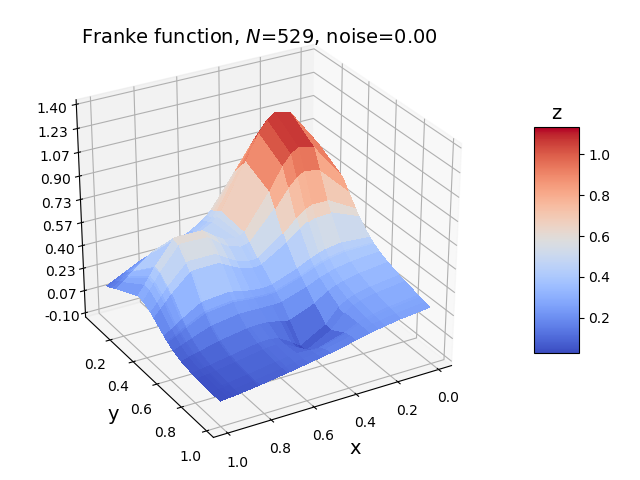
\includegraphics[scale=0.6]{../figures/task_a/surf_franke_N529_nf23_p5_noise0.00_seed4155.png}
	\caption{Example of the Franke function with no noise, with 529 randomly drawn points where $x,y \in [0,1]$.}
	\label{fig:franke_nonoise}
\end{figure}
%
We start the regression analysis by performing the OLS method on the data set. Table \ref{tab:franke_a} shows the MSE and R2 score for the train and test set where $p=5$, $N=529$. For this polynomial degree, both the training and test set shows good results, indicating that there is no significant overfitting.
\begin{table}[H]
  \centering
  \caption{Mean squared error and R2 score for the Franke function training and test set when $p=5$, $N=529$, and noise $\sigma = 0.05$}
  \label{tab:franke_a}
  \begin{tabular}{c|c|c}
    Data set & MSE & R2\\\hline
    train & 0.003334 & 0.949904\\
    test & 0.004674 & 0.929855
    \end{tabular}
\end{table}
The 95\% confidence intervals for $\beta_{\text{OLS}}$ is shown in figure \ref{fig:confbetaOLS}, with the same parameters. The confidence intervals are quite close to the coefficients, which makes sense given the MSE and R2 scores we found earlier.
\begin{figure}[H]
	\centering
	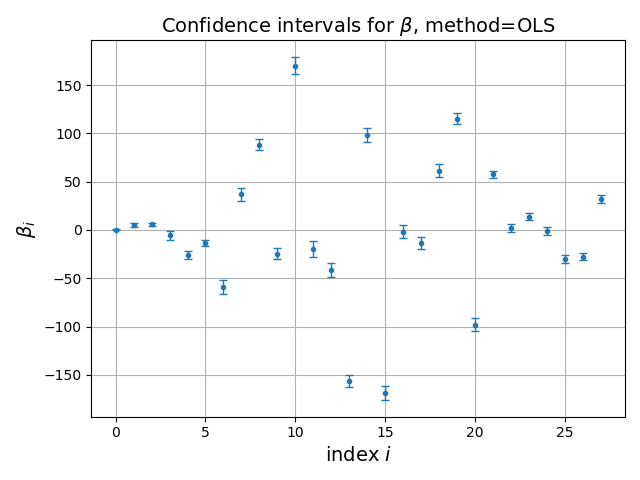
\includegraphics[scale=0.5]{../figures/task_a/beta_conf_int_OLS_N529_nf23_p6_noise0.05_seed4155_beta28.png}
	\caption{95\% confidence intervals for the regression coefficients $\beta_{\text{OLS}}$ for $p=6$, $N=529$, and noise $\sigma=0.05$.}
	\label{fig:confbetaOLS}
\end{figure}
To study how the model is affected by the degree $p$, we study the bias-variance trade-off by employing the Bootstrap resampling method. Now, we will be studying all three regression methods, OLS, Ridge and Lasso to make comparing easier. 
Figure \ref{fig:bias_var} shows the bias-variance trade-off for all three methods, with the Ridge and Lasso ones corresponding to the $\lambda$ that gave the lowest MSE. We see that for the OLS, once we go beyond $p=7$, the error and variance skyrockets. For Ridge and Lasso however, everything is fairly stable for $p>5$. This shows the effect of the regularization parameter $\lambda$, keeping the variance from exploding, and avoiding overfitting.
\begin{figure}[H]
  \centering
  \begin{subfigure}{0.49\textwidth}
    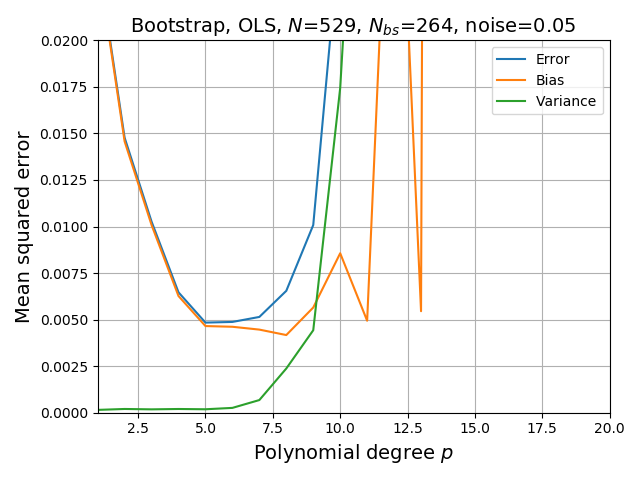
\includegraphics[scale=0.45]{../figures/task_b/bias_variance_N529_pmax20_nlamb1_noise0.05_seed4155_OLS_boot_Nbs264.png}
    \caption{OLS}
  \end{subfigure}
  \begin{subfigure}{0.49\textwidth}
    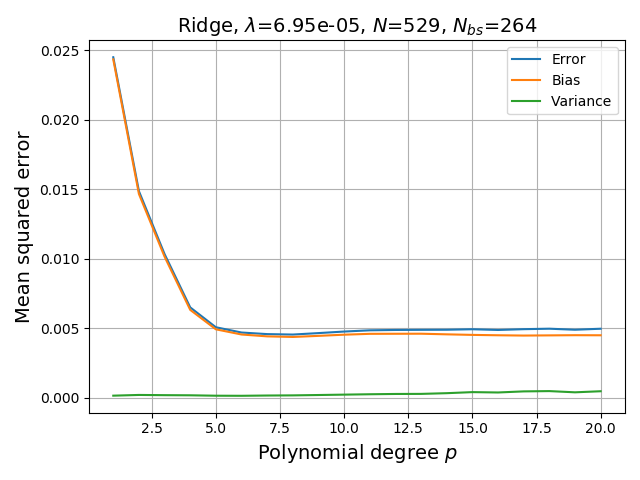
\includegraphics[scale=0.45]{../figures/task_d/bias_variance_N529_pmax20_nlamb20_noise0.05_seed4155_Ridge_boot_Nbs264_opt1.png}
    \caption{Ridge}
  \end{subfigure}\\
  \begin{subfigure}{0.49\textwidth}
    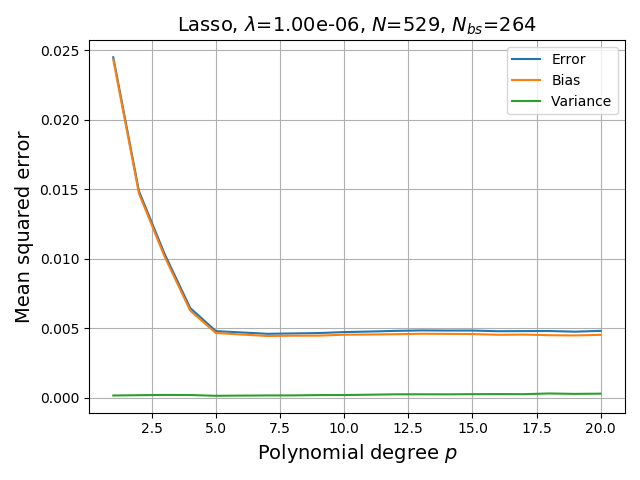
\includegraphics[scale=0.45]{../figures/task_e/bias_variance_N529_pmax20_nlamb10_noise0.05_seed4155_Lasso_boot_Nbs264_opt1.png}
    \caption{Lasso}
  \end{subfigure}
  \caption{Bias-variance plots for OLS, Ridge, and Lasso regression, where $N=529$, $\sigma = 0.05$ and $N_{\text{bs}} = N/2$. The best-fit hyperparameter for Ridge was found to be $\lambda = 2.98\cdot10^{-5}$, and $\lambda = 3.16\cdot10^{-5}$ for Lasso.}
  \label{fig:bias_var}
\end{figure}
Figure \ref{fig:app_Nbs} in appendix \ref{app:Frankeplots} shows how the OLS results depend on the number of bootstraps. The figure also is run with double the amount of data points, showing that the general shape is very similar, though the overfitting starts at slightly higher degree $p$. This is expected, as a with more data points, as there is more complexity in the data set. Also in the appendix, figure \ref{fig:beta_ridge} shows the 95\% confidence intervals of $\beta$ for Ridge regression, which compared to the OLS confidence intervals shown in figure \ref{fig:confbetaOLS} appear to be slightly larger.\\\\
Before looking closer at the hyperparameters $\lambda$, we look at the results from the $k$-fold Cross-validation. Figure \ref{fig:train_test_franke} shows the difference between the training and test MSE for all regression methods and both Bootstrap and Cross-validation. We see that CV gives very similar results to the Bootstrap, with some discrepancies. For OLS, the test MSE starts shooting up a lot later than for the Bootstrap results. For Ridge, the test MSE lies a lot closer to the training set up until $p=15$, where it starts going slightly up. Finally, Lasso in general is closer to the training MSE.
\begin{figure}[H]
  \centering
  \begin{subfigure}{0.49\textwidth}
    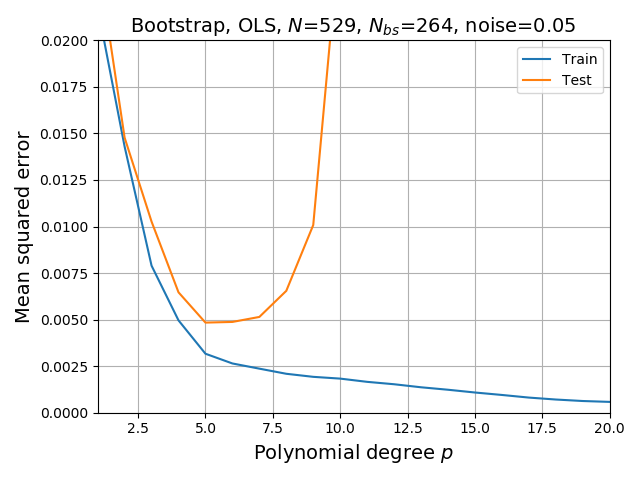
\includegraphics[scale=0.45]{../figures/task_b/MSE_train_test_Bootstrap_train_test_N529_pmax20_nlamb1_noise0.05_seed4155_OLS_boot_Nbs264.png}
    \caption{OLS - Bootstrap}
  \end{subfigure}
  \begin{subfigure}{0.49\textwidth}
    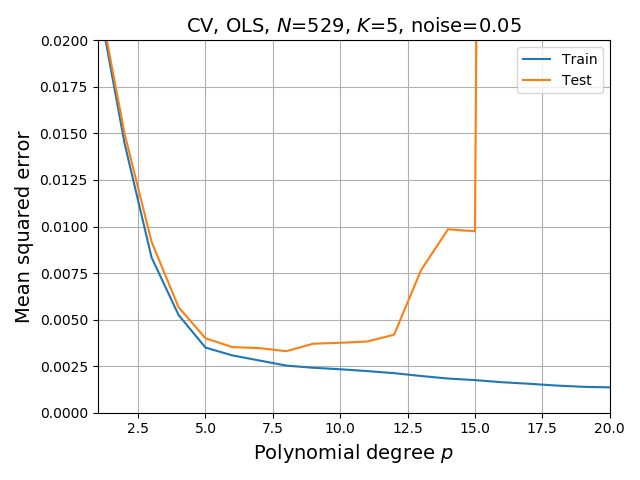
\includegraphics[scale=0.45]{../figures/task_b/MSE_train_test_CV_train_test_N529_pmax20_nlamb1_noise0.05_seed4155_OLS_cv_k5.png}
    \caption{OLS - Cross-validation}
  \end{subfigure}\\
  \begin{subfigure}{0.49\textwidth}
    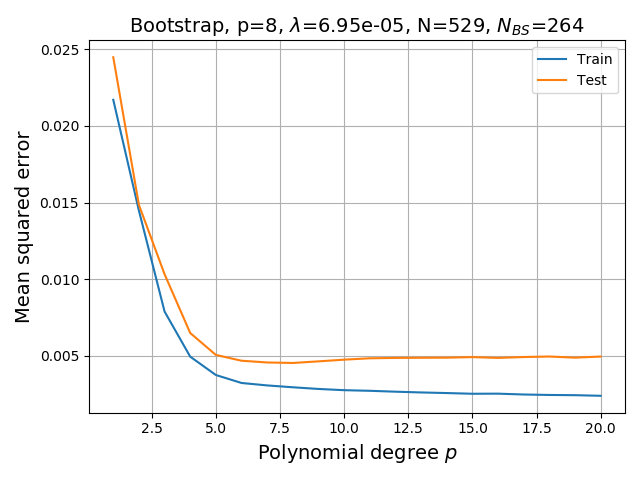
\includegraphics[scale=0.45]{../figures/task_d/MSE_train_test_Bootstrap_N529_pmax20_nlamb20_noise0.05_seed4155_Ridge_boot_Nbs264_opt1.png}
    \caption{Ridge - Bootstrap}
  \end{subfigure}
  \begin{subfigure}{0.49\textwidth}
    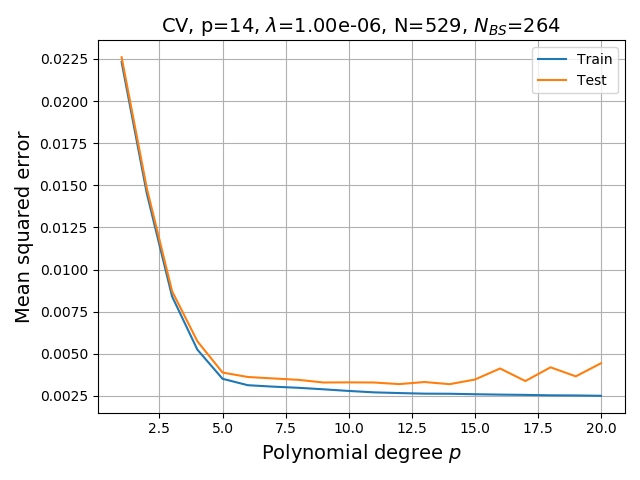
\includegraphics[scale=0.45]{../figures/task_d/MSE_train_test_CV_N529_pmax20_nlamb20_noise0.05_seed4155_Ridge_cv_k5_opt1.png}
    \caption{Ridge - Cross-validation}
  \end{subfigure}\\
  \begin{subfigure}{0.49\textwidth}
    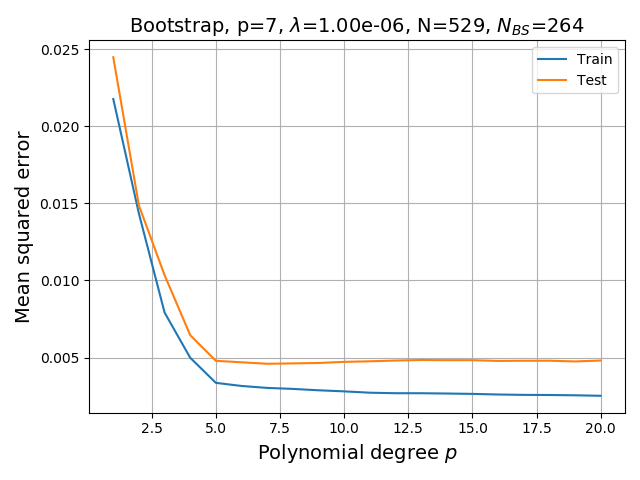
\includegraphics[scale=0.45]{../figures/task_e/MSE_train_test_Bootstrap_N529_pmax20_nlamb10_noise0.05_seed4155_Lasso_boot_Nbs264_opt1.png}
    \caption{Lasso - Bootstrap}
  \end{subfigure}
  \begin{subfigure}{0.49\textwidth}
    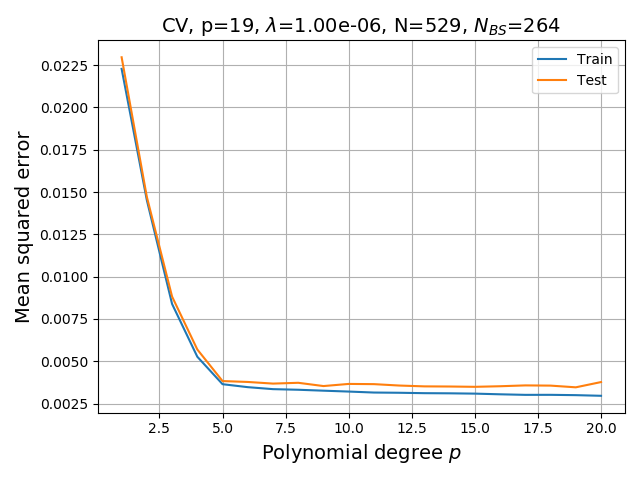
\includegraphics[scale=0.45]{../figures/task_e/MSE_train_test_CV_N529_pmax20_nlamb10_noise0.05_seed4155_Lasso_cv_k5_opt1.png}
    \caption{Lasso - Cross-validation}
  \end{subfigure}\\  
  \caption{Bias-variance plots for OLS, Ridge, and Lasso regression, where $N=529$, $\sigma = 0.05$ and $N_{\text{bs}} = N/2$. The best-fit hyperparameter for Ridge was found to be $\lambda = 2.98\cdot10^{-5}$, and $\lambda = 3.16\cdot10^{-5}$ for Lasso. The $p$-value on the Ridge + CV panel should have been the $p$-value corresponding to the minimum MSE value, but for some reason it is wrong.}
  \label{fig:train_test_franke}
\end{figure}
One way of looking at the hyperparameters would be to look at the heat map from all the values of $p$ and $\lambda$ that we used. Figure \ref{fig:franke_heatmap} shows the MSE heat map for Ridge and Lasso using Bootstrap. Heat maps for the bias, variance, and MSE from CV can be found in the Github repository \cite{Github1}. It is clear that the model prefers lower $\lambda$, though for high model complexity/polynomial degree a slightly higher $\lambda$ is preferred. Ridge has a slightly larger space of parameters that give good results, while the Lasso results start getting worse faster as $\lambda$ is increased.%While for Ridge, a large amount of the $\lambda$s give a good result, for Lasso the MSE almost always increase as $\lambda$ is increased. 
\begin{figure}[H]
  \centering
  \begin{subfigure}{0.49\textwidth}
    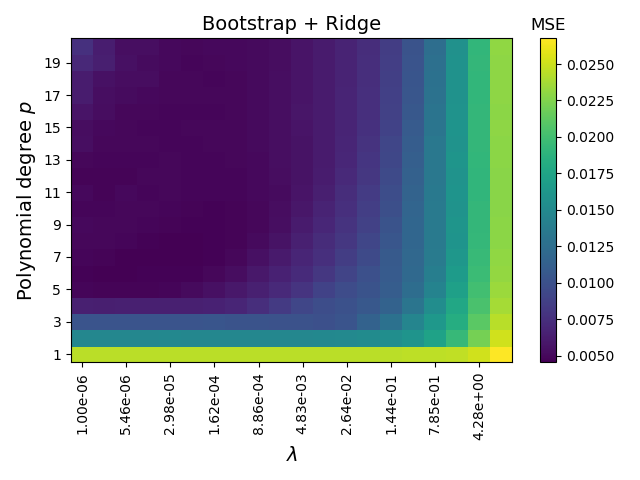
\includegraphics[scale=0.45]{../figures/task_d/heatmap_bs_error_N529_pmax20_nlamb20_noise0.05_seed4155_Ridge_boot_Nbs264.png}
    \caption{Ridge}
  \end{subfigure}
  \begin{subfigure}{0.49\textwidth}
    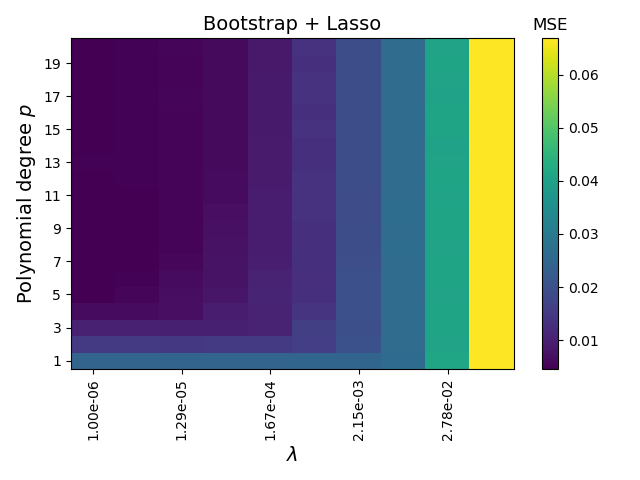
\includegraphics[scale=0.45]{../figures/task_e/heatmap_bs_error_N529_pmax20_nlamb10_noise0.05_seed4155_Lasso_boot_Nbs264.png}
    \caption{Lasso}
  \end{subfigure}
  \caption{Heat maps showing the MSE plotted against polynomial degree $p$ and the hyperparameter $\lambda$ for both Ridge and Lasso, using Bootstrap resampling. For Ridge, we calculated the results for 20 log-spaced $\lambda$s between $1\cdot10^{-6}$ and $1\cdot10^{1}$, while for Lasso we calculated 10 values of $\lambda$ between $1\cdot10^{-6}$ and $1\cdot10^{-1}$.}
  \label{fig:franke_heatmap}
\end{figure}
Figure \ref{fig:franke_lambdap} shows $\lambda_{\text{min}}$ plotted against $p$ for both Ridge and Lasso where $\lambda_{\text{min}}$ is the $\lambda$ corresponding to the lowest MSE for that polynomial degree. This is done both for Bootstrap and Cross-validation. For Ridge and Bootstrap, the optimal $\lambda$ varies quite a bit for each value of $p$, while for CV, it stays at the lowest value for $p \in [8, 12]$, where there is a peak in the Bootstrap. The axes are slightly different, so plotting them on top of each other would have been interesting.\\\\
For Lasso, the $\lambda$ value drops down to the lowest value at $p\sim3-4$ for both Bootstrap and CV, staying there until the end. This shows that we probably should have tried running with even lower values. Running with the starting point $\lambda = 1\cdot10^{-6}$ took extremely long time to converge (or just reach the maximum iteration count), so trying with any lower is not very tempting. 
\begin{figure}[H]
  \centering
  \begin{subfigure}{0.49\textwidth}
    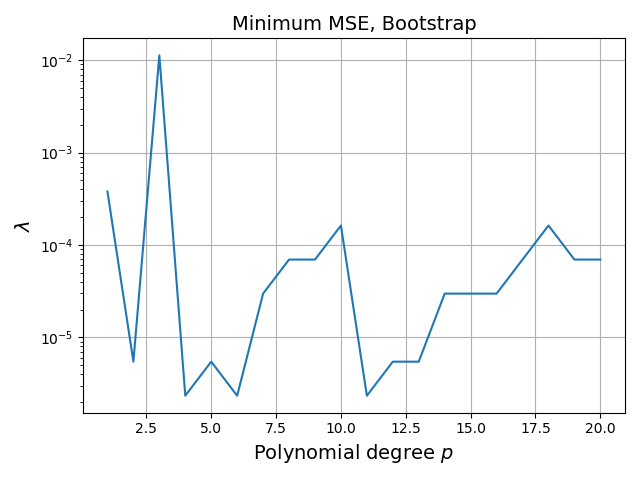
\includegraphics[scale=0.45]{../figures/task_d/degree_lambda_N529_pmax20_nlamb20_noise0.05_seed4155_Ridge_boot_Nbs264.png}
    \caption{Ridge - Bootstrap}
  \end{subfigure}
  \begin{subfigure}{0.49\textwidth}
    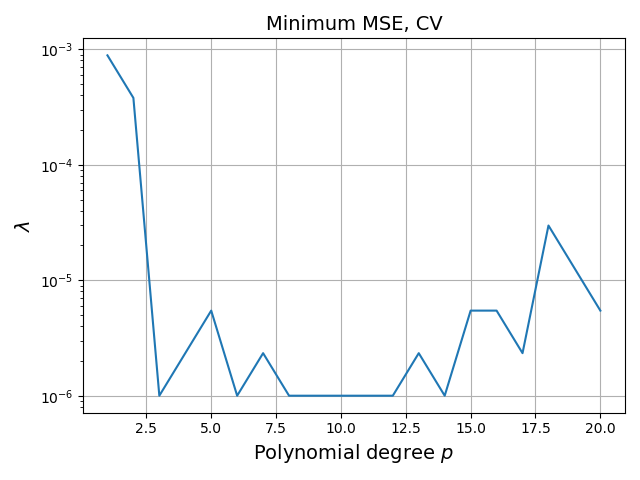
\includegraphics[scale=0.45]{../figures/task_d/degree_lambda_N529_pmax20_nlamb20_noise0.05_seed4155_Ridge_cv_k5.png}
    \caption{Ridge - Cross-validation}
  \end{subfigure}\\
  \begin{subfigure}{0.49\textwidth}
    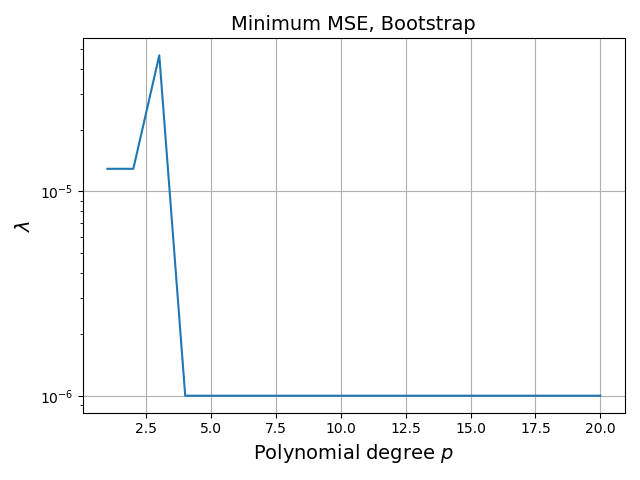
\includegraphics[scale=0.45]{../figures/task_e/degree_lambda_N529_pmax20_nlamb10_noise0.05_seed4155_Lasso_boot_Nbs264.png}
    \caption{Lasso - Bootstrap}
  \end{subfigure}
  \begin{subfigure}{0.49\textwidth}
    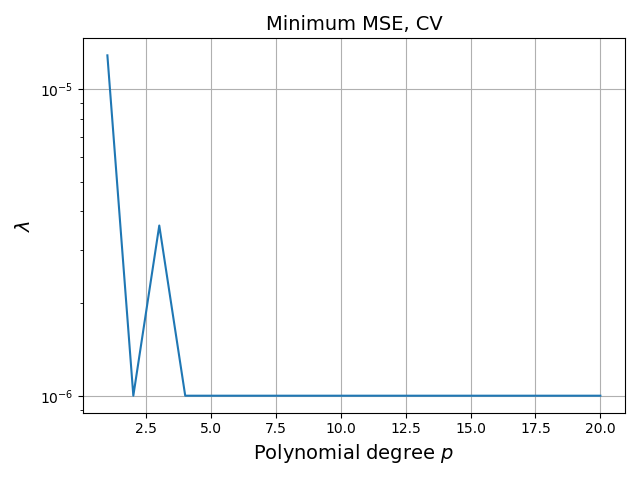
\includegraphics[scale=0.45]{../figures/task_e/degree_lambda_N529_pmax20_nlamb10_noise0.05_seed4155_Lasso_cv_k5.png}
    \caption{Lasso - Cross-validation}
  \end{subfigure}
  \caption{Hyperparameter $\lambda$ plotted against polynomial degree $p$ for Ridge/Lasso regression with Bootstrap/Cross-validation. The $\lambda$ value corresponds to the one that gives the lowest MSE value at the given $p$.}
  \label{fig:franke_lambdap}
\end{figure}
Finally, table \ref{tab:best_fit_franke} shows the best-fit parameters $p$ and $\lambda$ for each of the three regression methods, and for each of the resampling methods. For both Bootstrap and Cross-validation, Ridge regression seems to be the best option, with both OLS and Lasso only slightly behind. For the Bootstrap, Lasso performs better than OLS, while for CV, OLS performs better. Looking at the R2 scores could have been useful to see how significant those differences are, but based on the train/test MSE plots in figure \ref{fig:train_test_franke}, the differences are fairly small. Worth noting out is that while Ridge and Lasso are very similar results wise, Ridge is quite a bit faster, as Lasso can be extremely slow since there is no analytical solution. OLS on the other hand is even faster than Ridge, but has a significant disadvantage when it comes to stability. As shown with both the bias-variance trade-off and train-test plots, Ridge and Lasso has a much wider range of parameters that give good results, as the hyperparameter suppresses the overfitting problem with OLS.
\begin{table}[H]
  \centering
  \caption{The best-fit parameters for OLS, Ridge and Lasso regression given the lowest MSE value. First three columns is the Bootstrap, last three is Cross-validation}
  \label{tab:best_fit_franke}
  \begin{tabular}{c|c|c|c||c|c|c}
    Reg. method & p (BS)& $\lambda$ (BS) & MSE (BS) & p (CV) & $\lambda$ (CV) & MSE (CV) \\\hline
    OLS & 5 & - & $4.84\cdot10^{-3}$ & 8 & - & $3.30\cdot10^{-3}$\\
    Ridge & 8 & $6.95\cdot10^{-5}$ & $4.55\cdot10^{-3}$ & 15 & $5.46\cdot10^{-6}$ & $3.28\cdot10^{-3}$\\
    Lasso & 7 & $1.00\cdot10^{-6}$ &$4.59\cdot10^{-3}$ & 19 & $1.00\cdot10^{-6}$ & $3.46\cdot10^{-3}$
    \end{tabular}
\end{table}
Before moving on to the terrain data, to point out that for some reason the $p$ and $\lambda$ values present in the title of figure \ref{fig:train_test_franke} for the CV+Ridge panel specifically for some reason is incorrect. Quite a bit of time was spent looking at the code and output files without understanding why that one specifically is wrong.
\subsection{Terrain data}
We look at the terrain map described in chapter \ref{sec:data_sets}. The entire map is $3601\times1801$ data points, so performing the analysis on the entire map is outside of the scope of this project, so instead we will be focusing on a smaller region of the map. Ideally, we would have performed this analysis on many patches of the map, but sadly due to time constraints we will only have the results for this one patch. Altering which area and the size of it is relatively easy in the code, should one desire to test it out.\\\\
Figure \ref{fig:terrain_patch} shows the zoomed in map and a 3D surface plot of the patch we will be studying in this section. First, we normalize the map by the maximum height in the dataset, and choose a $150\times150$ grid for our region, giving us a data set of size 22500 samples, quite a bit more than we had for the Franke function. The region we chose is located at $(x,y)$ $(880, 2920)$ to $(1030, 3070)$, and the center of the map corresponds roughly to where the author grew up. Beyond that, the area consists of several fairly sharp mountains/hills and decent variation in the features.
\begin{figure}[H]
  \centering
  \begin{subfigure}{0.79\textwidth}
  	\centering
    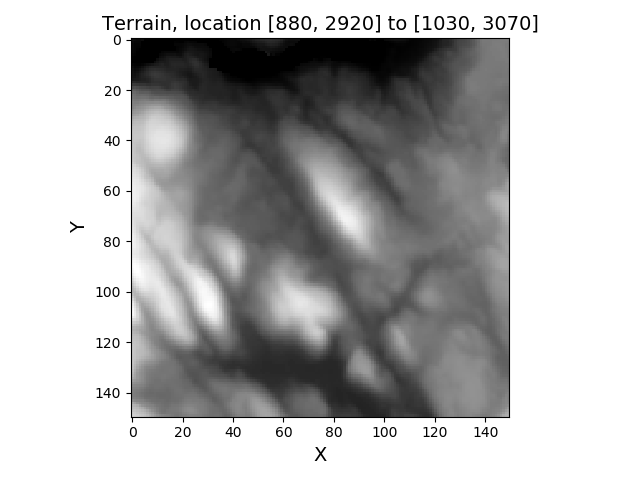
\includegraphics[scale=0.60]{../figures/task_f/terrain_n150_880_2920.png}
    \caption{Terrain}
  \end{subfigure}\\
  \begin{subfigure}{0.79\textwidth}
  	\centering
    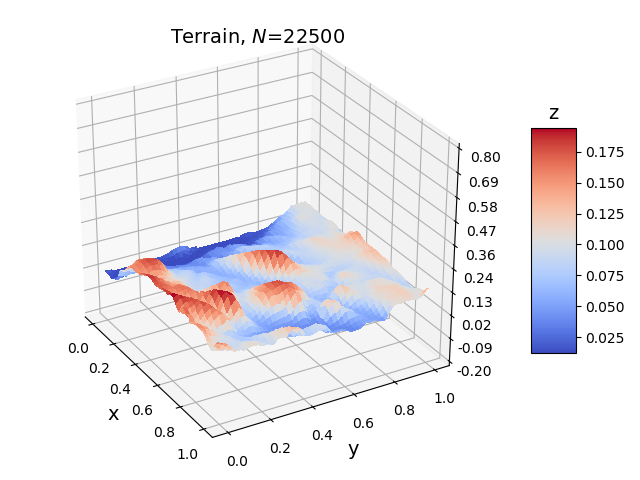
\includegraphics[scale=0.60]{../figures/task_f/surf_surf_terrain_n150_880_2920.png}
    \caption{3D surface plot}
  \end{subfigure}
  \caption{Top: Zoomed in view of the map. Bottom: 3D surface plot of the same region. The region we are studying is located at $(x,y)$ $(880, 2920)$ to $(1030, 3070)$, with $N=22500$ samples.}
  \label{fig:terrain_patch}
\end{figure}
Figure \ref{fig:bias_var_terrain} shows the bias-variance trade-off for all regression methods using Bootstrap. The OLS keeps decreasing as the degree increases, and seems to have a lower error than both Ridge and Lasso for roughly $p>11$. Since we have so many data points, it might be that the OLS does not yet start overfitting, and possibly the noise level of the data is low enough to push this threshold further up. Testing with higher values of $p$ would probably be the way forward, but doing so takes significantly more time, as the number of terms in the design matrix keeps increasing by $p+2$ for every new degree up you go, with 231 terms for $p=20$, 496 for $p=30$, 861 for $p=40$.
\begin{figure}[H]
  \centering
  \begin{subfigure}{0.49\textwidth}
    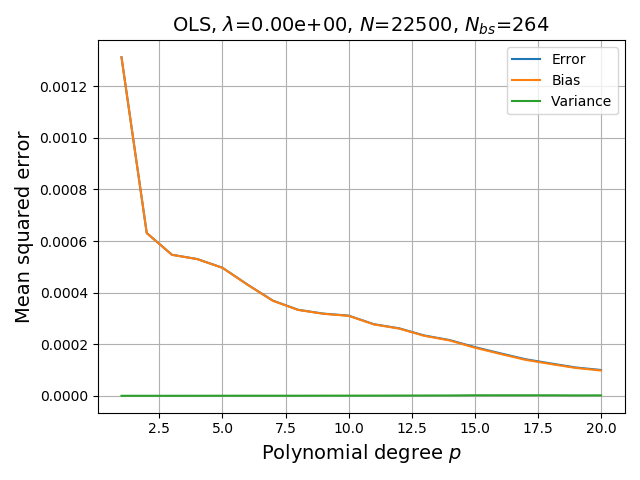
\includegraphics[scale=0.45]{../figures/task_g/OLS/bias_variance_N22500_patch1_pmax20_nlamb1_OLS_boot_Nbs264_opt1.png}
    \caption{OLS}
  \end{subfigure}
  \begin{subfigure}{0.49\textwidth}
    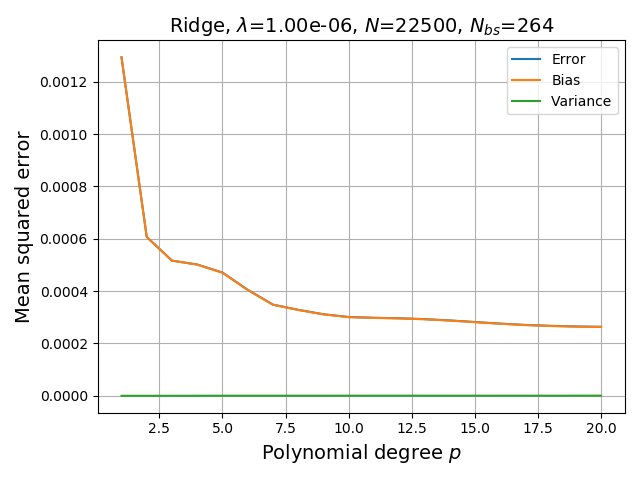
\includegraphics[scale=0.45]{../figures/task_g/Ridge/bias_variance_N22500_patch1_pmax20_nlamb15_Ridge_boot_Nbs264_opt1.png}
    \caption{Ridge}
  \end{subfigure}\\
  \begin{subfigure}{0.49\textwidth}
%    \includegraphics[scale=0.45]{../figures/task_g/Ridge/%bias_variance_N22500_patch1_pmax20_nlamb15_Ridge_boot_Nbs100_opt1.png}
    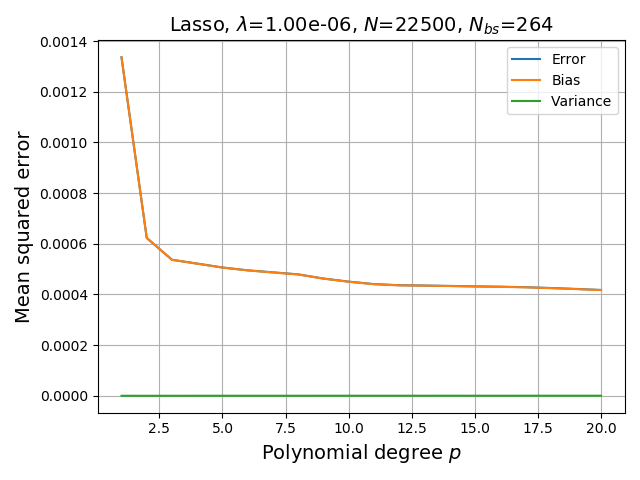
\includegraphics[scale=0.45]{../figures/task_g/Lasso/bias_variance_N22500_patch1_pmax20_nlamb15_Lasso_boot_Nbs264_opt1.png}
    \caption{Lasso}
  \end{subfigure}
  \caption{Bias-variance plots for OLS, Ridge, and Lasso regression, for the terrain patch, $N=22500$, $N_{\text{bs}} = 264$.}%The best-fit hyperparameter for Ridge was found to be $\lambda = 2.98\cdot10^{-5}$, and $\lambda = 3.16\cdot10^{-5}$ for Lasso.}
  \label{fig:bias_var_terrain}
\end{figure}
Figure \ref{fig:mse_testcomp_terrain} shows the direct comparison between the test MSE from Bootstrap and Cross-validation, computed for each of the regression methods. We see that the results are quite close, with Bootstrap giving a slightly lower error for higher $p$-values for Ridge, which contrasts the results for the Franke function where Cross-validation gave a lower test error than Bootstrap, though the difference for the terrain data is much smaller than it was for the Franke function. For OLS and Lasso, Bootstrap has a slightly higher error than CV.
\begin{figure}[H]
  \centering
  \begin{subfigure}{0.49\textwidth}
    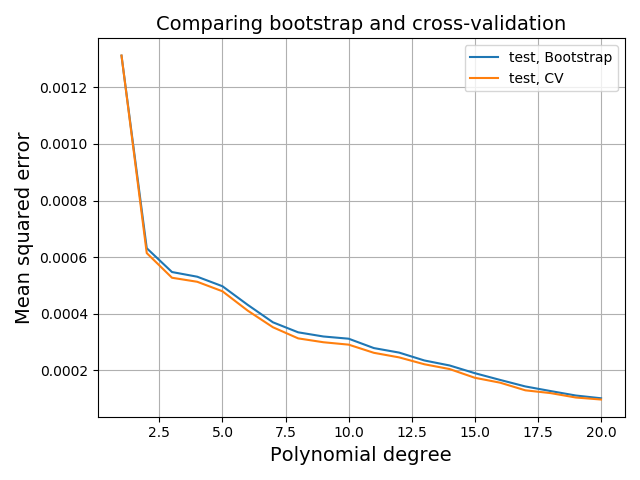
\includegraphics[scale=0.45]{../figures/task_g/OLS/test_compare_BS_CV_p20_N22500_patch1_pmax20_nlamb1_OLS_Nbs264_k5_opt1.png}
    \caption{OLS}
  \end{subfigure}
  \begin{subfigure}{0.49\textwidth}
    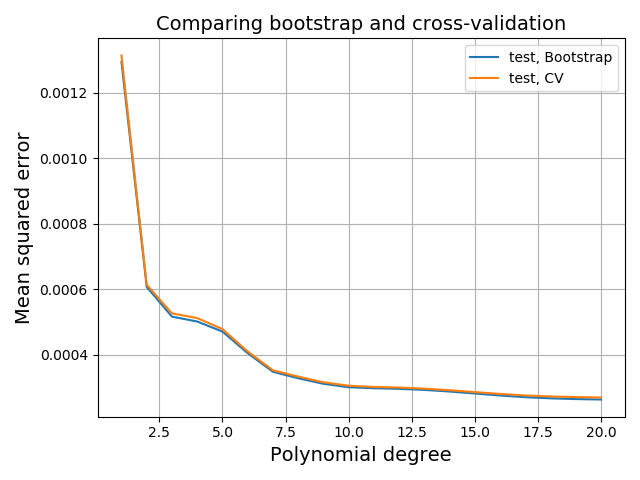
\includegraphics[scale=0.45]{../figures/task_g/Ridge/test_compare_BS_CV_p20_N22500_patch1_pmax20_nlamb15_Ridge_Nbs264_k5_opt1.png}
    \caption{Ridge}
  \end{subfigure}\\
  \begin{subfigure}{0.49\textwidth}
%    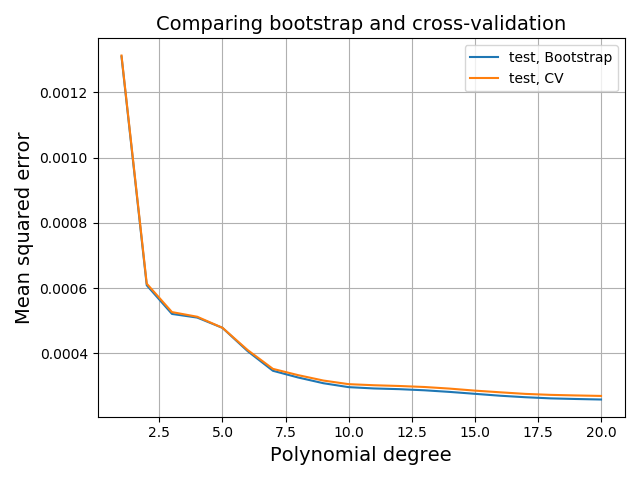
\includegraphics[scale=0.45]{../figures/task_g/Ridge/test_compare_BS_CV_p20_N22500_patch1_pmax20_nlamb15_Ridge_Nbs100_k5_opt1.png}
    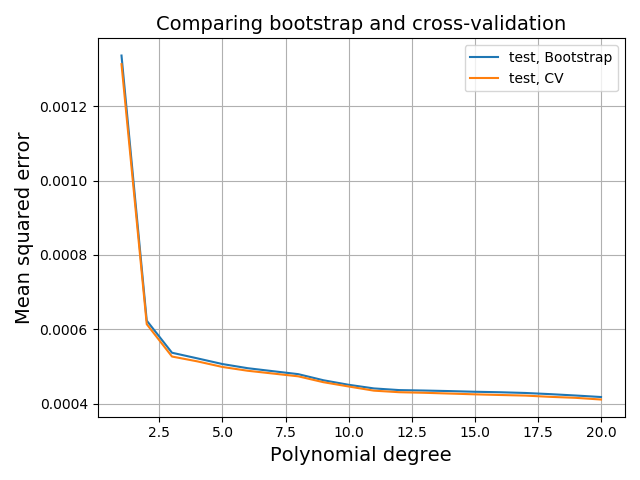
\includegraphics[scale=0.45]{../figures/task_g/Lasso/test_compare_BS_CV_p20_N22500_patch1_pmax20_nlamb15_Lasso_Nbs264_k5_opt1.png}
    \caption{Lasso}
  \end{subfigure}
  \caption{Comparison between the test MSE from Bootstrap and Cross-validation, for each regression method. Data set is the terrain data described earlier, $N=22500$, $N_{\text{bs}} = 264$.}
  \label{fig:mse_testcomp_terrain}
\end{figure}
To study the hyperparameter, we again start by plotting the heat maps for Ridge and Lasso. Figure \ref{fig:terrain_heatmap} shows the MSE heat maps when using Bootstrap. The Cross-validation results can be found in appendix \ref{app:terrainplots}, figure \ref{fig:terrain_heatmap_CV}. We see that the Ridge results shows a smaller dependence on the hyperparameter compared to the Franke function, as even the highest $\lambda$s give decent results. For Lasso, the results are more in line with the Franke function, with a much smaller range of viable $\lambda$ values. Note the difference in the $x$-axis range.
\begin{figure}[H]
  \centering
  \begin{subfigure}{0.49\textwidth}
    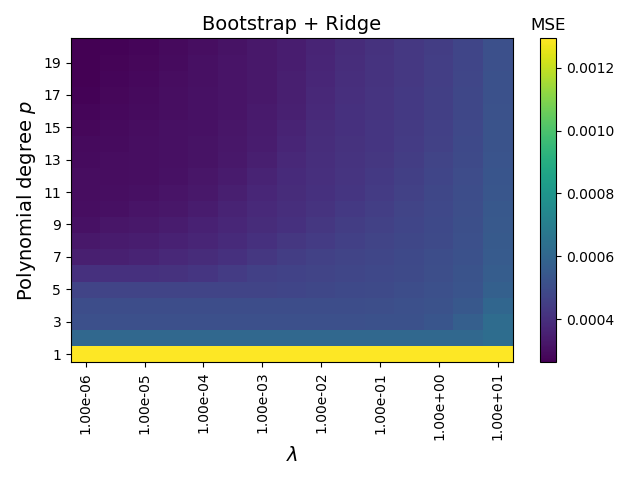
\includegraphics[scale=0.45]{../figures/task_g/Ridge/heatmap_bs_error_N22500_patch1_pmax20_nlamb15_Ridge_boot_Nbs264.png}
    \caption{Ridge}
  \end{subfigure}
  \begin{subfigure}{0.49\textwidth}
    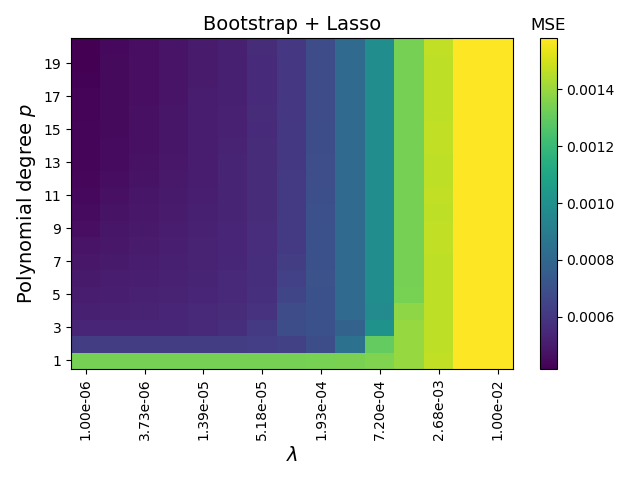
\includegraphics[scale=0.45]{../figures/task_g/Lasso/heatmap_bs_error_N22500_patch1_pmax20_nlamb15_Lasso_boot_Nbs264.png}
    \caption{Lasso}
  \end{subfigure}
  \caption{Heat maps showing the MSE plotted against polynomial degree $p$ and the hyperparameter $\lambda$ for both Ridge and Lasso, using Bootstrap resampling. For Ridge, we calculated the results for 15 log-spaced $\lambda$s between $1\cdot10^{-6}$ and $1\cdot10^{1}$, while for Lasso we calculated 15 values of $\lambda$ between $1\cdot10^{-6}$ and $1\cdot10^{-2}$. $N_{\text{bs}} = 264$.}
  \label{fig:terrain_heatmap}
\end{figure}

Figure \ref{fig:terrain_lambdap} shows $\lambda_{\text{min}}$ plotted against $p$ for both Ridge and Lasso where $\lambda_{\text{min}}$ is the $\lambda$ corresponding to the lowest MSE for that polynomial degree. This is done both with both Bootstrap and CV, but only Bootstrap is shown here since they show the same trends. We see that both Ridge and Lasso goes towards the minimum $\lambda$ value and stays there as $p$ is increased. This happens faster for Lasso regression at $p=3$, and $p=7$ for Ridge.
\begin{figure}[H]
  \centering
  \begin{subfigure}{0.49\textwidth}
    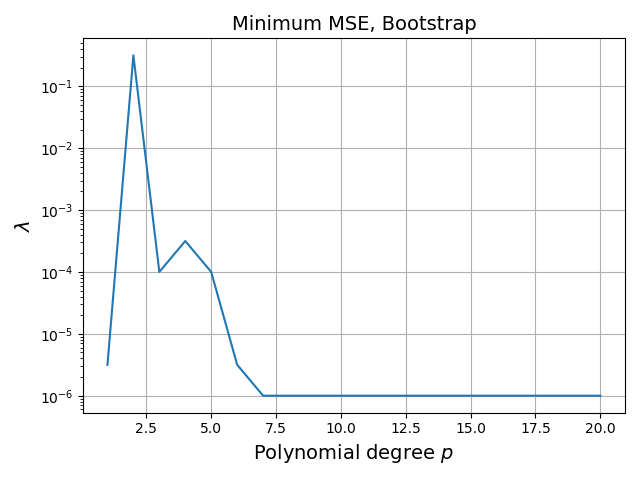
\includegraphics[scale=0.45]{../figures/task_g/Ridge/degree_lambda_N22500_patch1_pmax20_nlamb15_Ridge_boot_Nbs264.png}
    \caption{Ridge - Bootstrap}
  \end{subfigure}
  \begin{subfigure}{0.49\textwidth}
    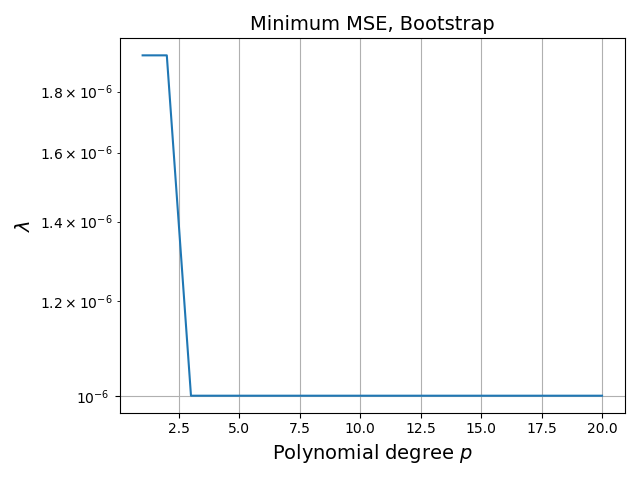
\includegraphics[scale=0.45]{../figures/task_g/Lasso/degree_lambda_N22500_patch1_pmax20_nlamb15_Lasso_boot_Nbs264.png}
    \caption{Lasso - Bootstrap}
  \end{subfigure}
  \caption{Hyperparameter $\lambda$ plotted against polynomial degree $p$ for Ridge/Lasso regression with Bootstrap. The $\lambda$ value corresponds to the one that gives the lowest MSE value at the given $p$.}
  \label{fig:terrain_lambdap}
\end{figure}
Finally, we summarize our results for the terrain data in a table. Table \ref{tab:best_fit_terrain} shows the optimal ($p$, $\lambda$) values and the corresponding MSE value for all three regression methods and both resampling methods. Unsurprisingly, all the $p$ values end up being $p=20$, the highest model complexity, which fits what we observed in figure \ref{fig:bias_var_terrain} and figure \ref{fig:mse_testcomp_terrain}. Beyond that, we see that OLS gives the best result for the terrain data by a decent margin. Lasso performs the worst of the bunch, with a similar difference to Ridge as was between OLS and Ridge. We also see that Bootstrap and Cross-validation give very similar results, being much closer to each other compared to earlier with the Franke function.
\\\\
It is clear that in order to properly evaluate the regression methods, a higher $p$ value is needed, which sadly is difficult to do time wise. Also, in order to do so, it would probably be a good idea to try to optimize the code in order to speed up some of the loops, and potentially parallelizing some of them. It would also be ideal to try to test out more regions of the map and not just this one, to see if perhaps a region that is more uneven yields different results.
\begin{table}[H]
  \centering
  \caption{The best-fit parameters for OLS, Ridge and Lasso regression for the terrain patch, given the lowest MSE value. First three columns is the Bootstrap, last three is Cross-validation.}
  \label{tab:best_fit_terrain}
  \begin{tabular}{c|c|c|c||c|c|c}
    Reg. method & p (BS)& $\lambda$ (BS) & MSE (BS) & p (CV) & $\lambda$ (CV) & MSE (CV) \\\hline
    OLS & 20 & - & $1.00\cdot10^{-4}$ & 20 & - & $9.58\cdot10^{-5}$\\
    Ridge & 20 & $1.00\cdot10^{-6}$ & $2.64\cdot10^{-4}$ & 20 & $1.00\cdot10^{-6}$ & $2.70\cdot10^{-4}$\\
    Lasso & 20 & $1.00\cdot10^{-6}$ &$4.18\cdot10^{-4}$ & 20 & $1.00\cdot10^{-6}$ & $4.11\cdot10^{-4}$
    \end{tabular}
\end{table}
%%%%%%%%%%%%%%%%%%%%%%%%%%%%%%%%%%%%%%%%%%%%%%%%%%%%%%%%%%%%%%%%%%%%%%%%%%%%%%%%%%%%%%%%%%
%%%%%%%%%%%%%%%%%%%%%%%%%%%%%%%%%%%%%%%%%%%%%%%%%%%%%%%%%%%%%%%%%%%%%%%%%%%%%%%%%%%%%%%%%%
\section{Conclusion} \label{chap:conclusion}
In this project, we set out to investigate how different methods of linear regression performs on the Franke function, as well as terrain elevation data. To assess our models, we employed Bootstrap and Cross-validation as resampling methods.
\\\\
For the Franke function, we found that all three methods, OLS, Ridge and Lasso performed very similarly, giving errors on the scale $10^{-3}$ for the best-fit model. Ridge was however the best model, both in accuracy and stability. Lasso yielded almost as good results as Ridge, but was significantly slower as it has no analytical solution. Cross-validation gave the lowest errors, with roughly 30\% improvement over Bootstrapping for the best-fit models.
%Introduce why we set out, then explain results
\\\\
For the terrain data, we found that the OLS performed the best, with Ridge being a decent bit behind, and Lasso roughly as much behind Ridge. The best fit for OLS was at $p=20$, which gave an MSE of $9.58\cdot10^{-5}$. In this case, Cross-validation was only marginally better for OLS and Lasso regression, and slightly worse for Ridge, but the difference is minor. As all the best fits was the highest $p$-value we tested, testing higher polynomial degrees would be necessary.
\\\\
For future work, looking closer at the terrain data would probably be a good idea. Ideally, more parts of the maps should be checked instead of just one small patch, in order to see how more complex and noisy regions affect the results, as well as increasing the degrees that are tested (and the hyperparameter $\lambda$). This however would take significantly more time, especially for Lasso, so looking into parallelizing the analysis would be relevant. Since all $p$ and $\lambda$ computations are independent, doing so should not be too difficult.
%\red{middle?} For future work, it would have been worth parallelizing parts of the code. Could be either the polynomial degrees, the hyperparameters, or both the Bootstrap and Cross-validation parts of the code, as none of them directly depend on each other. The Lasso in scikit-learn however has the possibility to use previous results, so would need to check out where it is optimal for Lasso. CUDA cores
%For terrain, OLS performed well, but to say definite probalby would have needed to test more varied regions (and more at all)
%%%%%%%%%%%%%%%%%%%%%%%%%%%%%%%%%%%%%%%%%%%%%%%%%%%%%%%%%%%%%%%%%%%%%%%%%%%%%%%%%%%%%%%%%%
%%%%%%%%%%%%%%%%%%%%%%%%%%%%%%%%%%%%%%%%%%%%%%%%%%%%%%%%%%%%%%%%%%%%%%%%%%%%%%%%%%%%%%%%%%
\bibliography{references}
%%%%%%%%%%%%%%%%%%%%%%%%%%%%%%%%%%%%%%%%%%%%%%%%%%%%%%%%%%%%%%%%%%%%%%%%%%%%%%%%%%%%%%%%%%
%%%%%%%%%%%%%%%%%%%%%%%%%%%%%%%%%%%%%%%%%%%%%%%%%%%%%%%%%%%%%%%%%%%%%%%%%%%%%%%%%%%%%%%%%%
\appendix
\section*{Appendix} \label{chap:appendix}
%\section{Appendix} \label{chap:appendix}
\section{Data sets} \label{app:datasets}
\subsection{Franke function} \label{app:Franke}
The Franke function as given in \cite{Franke}
\begin{align*}
	f(x,y) &= \frac{3}{4}\exp\bigg(-\frac{(9x-2)^2}{4} - \frac{(9y-2)^2}{4}\bigg)
	+\frac{3}{4}\exp\bigg(-\frac{(9x+1)^2}{49} - \frac{(9y+1)^2}{10}\bigg)\\
	&+\frac{1}{2}\exp\bigg(-\frac{(9x-7)^2}{4} - \frac{(9y-3)^2}{4}\bigg)
	-\frac{1}{5}\exp\big(-(9x-4)^2 - (9y-7)^2\big)
\end{align*}
where $x,y \in [0, 1]$.

\subsection{Terrain data} \label{app:terrain}
\begin{figure}[H]
	\centering
	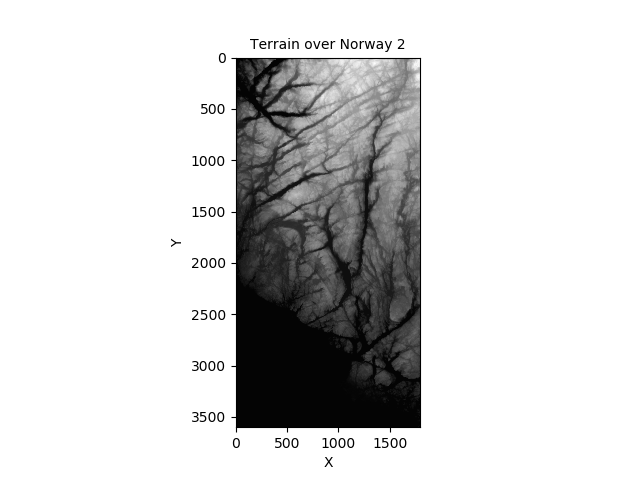
\includegraphics[scale=0.91]{../figures/task_f/entire_map.png}
	\caption{Plot of the entire terrain map in \texttt{SRTM\_data\_Norway\_3.tif}. Map is over a region south-east in Norway (Vestfold og Telemark, Viken). Coordinates $(x,y) = (1100, 3000)$ correspond to the location of the city Skien.}
	\label{fig:entiremap}
\end{figure}

%\section{Testing and verifying methods} \label{app:testing}

\section{Franke function plots} \label{app:Frankeplots}
\begin{figure}[H]
  \centering
  \begin{subfigure}{0.49\textwidth}
    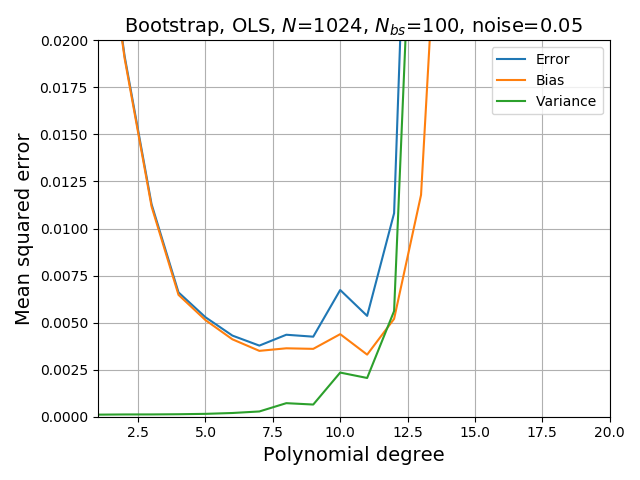
\includegraphics[scale=0.45]{../figures/task_b/bias_variance_N1024_pmax20_nlamb1_noise0.05_seed4155_OLS_boot_Nbs100.png}
    \caption{$N_{\text{bs}} = 100$}
  \end{subfigure}
  \begin{subfigure}{0.49\textwidth}
    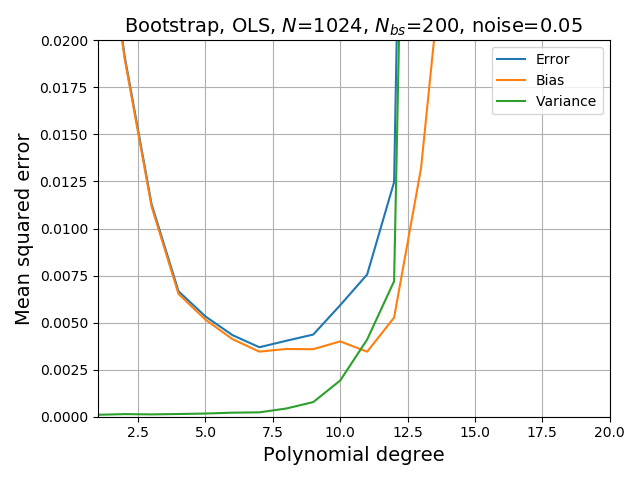
\includegraphics[scale=0.45]{../figures/task_b/bias_variance_N1024_pmax20_nlamb1_noise0.05_seed4155_OLS_boot_Nbs200.png}
    \caption{$N_{\text{bs}} = 200$}
  \end{subfigure}\\
  \begin{subfigure}{0.49\textwidth}
    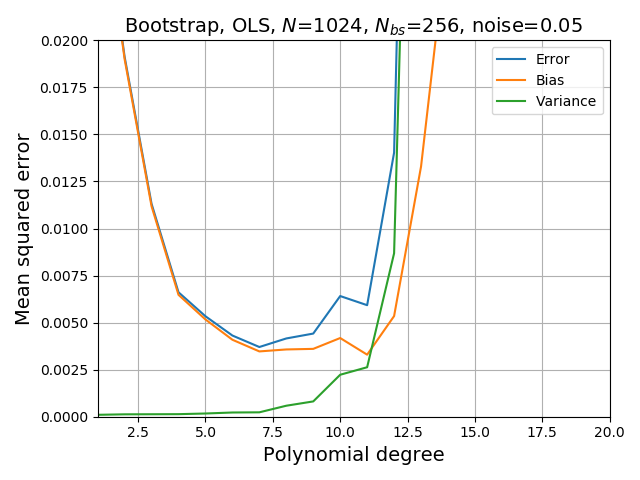
\includegraphics[scale=0.45]{../figures/task_b/bias_variance_N1024_pmax20_nlamb1_noise0.05_seed4155_OLS_boot_Nbs256.png}
    \caption{$N_{\text{bs}} = 256$}
  \end{subfigure}
  \begin{subfigure}{0.49\textwidth}
    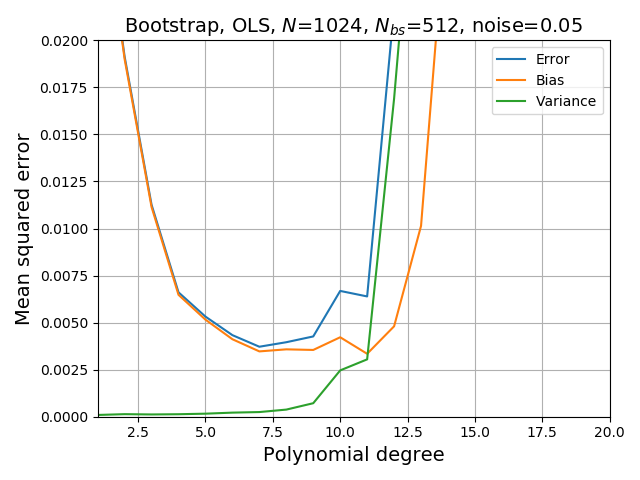
\includegraphics[scale=0.45]{../figures/task_b/bias_variance_N1024_pmax20_nlamb1_noise0.05_seed4155_OLS_boot_Nbs512.png}
    \caption{$N_{\text{bs}} = 512$}
  \end{subfigure}
  \caption{Bias-variance plots for OLS where the number of bootstraps $N_{\text{bs}}$ is varied. $N=1024$, $\sigma=0.05$. In general, all four produce very similar results.}
  \label{fig:app_Nbs}
\end{figure}

\begin{figure}[H]
	\centering
	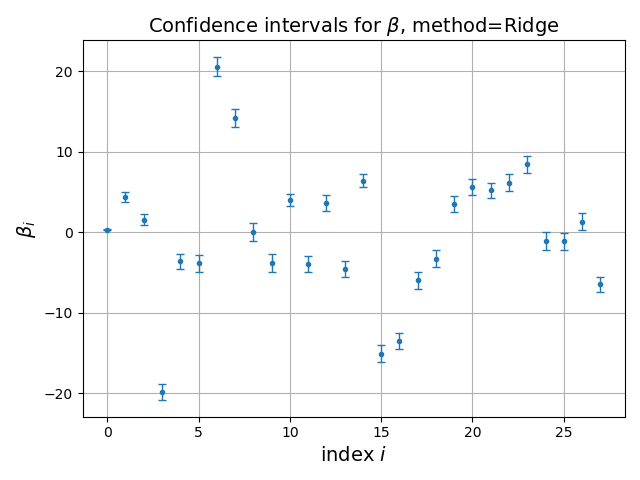
\includegraphics[scale=0.5]{../figures/task_d/beta_conf_int_Ridge_N529_pmax20_nlamb20_noise0.05_seed4155_beta28.png}
	\caption{95\% confidence intervals for the regression coefficients $\beta_{\text{Ridge}}$ for $p=6$, $N=529$, and noise $\sigma=0.05$.}
	\label{fig:beta_ridge}
\end{figure}
\section{Terrain data plots} \label{app:terrainplots}
%\subsubsection{Hyperpar
\begin{figure}[H]
  \centering
  \begin{subfigure}{0.49\textwidth}
    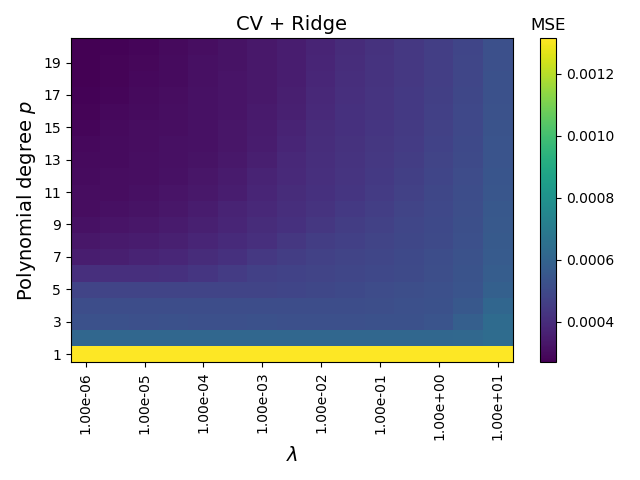
\includegraphics[scale=0.45]{../figures/task_g/Ridge/heatmap_cv_error_N22500_patch1_pmax20_nlamb15_Ridge_cv_k5.png}
    \caption{Ridge}
  \end{subfigure}
  \begin{subfigure}{0.49\textwidth}
    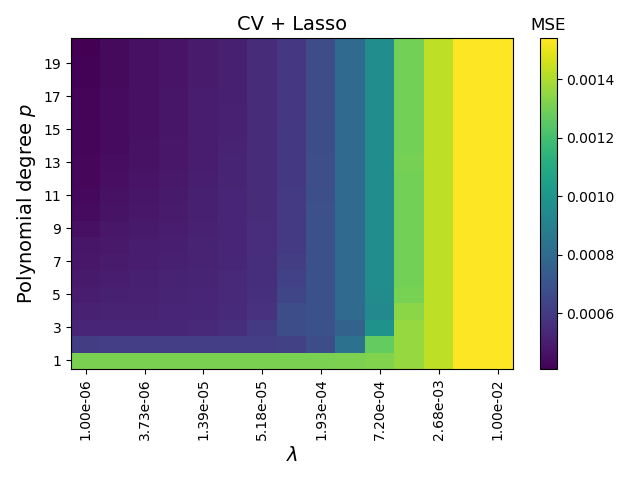
\includegraphics[scale=0.45]{../figures/task_g/Lasso/heatmap_cv_error_N22500_patch1_pmax20_nlamb15_Lasso_cv_k5.png}
    \caption{Lasso}
  \end{subfigure}
  \caption{Heat maps showing the MSE plotted against polynomial degree $p$ and the hyperparameter $\lambda$ for both Ridge and Lasso, using Cross-validation. For Ridge, we calculated the results for 15 log-spaced $\lambda$s between $1\cdot10^{-6}$ and $1\cdot10^{1}$, while for Lasso we calculated 15 values of $\lambda$ between $1\cdot10^{-6}$ and $1\cdot10^{-2}$. Plots are almost identical to the Bootstrap version found in figure \ref{fig:terrain_heatmap}.}
  \label{fig:terrain_heatmap_CV}
\end{figure}

\end{document}